\documentclass[]{article}

%opening
\title{Learning neural Question Answering Systems for Low-resource Langauges}
\author{C.W, R.H}

\usepackage{graphicx}

\begin{document}

\maketitle

\newpage
\begin{abstract}
ABSTRACT PLACEHOLDER
\end{abstract}

\newpage
\tableofcontents

\newpage
\section{Introduction}
Text understanding and question answering have always been among some of the most challenging tasks in natural language processing. With the rise of deep learning and DNN-based learning algorithms, as well as the increasing availability of large training datasets, neural network-based QA has been steadily gaining traction. A competent question answering system has a wide variety of practical uses in areas such as automated online self-service, intelligent web search, AI personal assistants etc. In recent years, many influential models have been proposed in this field, such as Memory Networks \cite{sukhbaatar2015end}, Dynamic Memory Networks \cite{kumar2016ask} and Differentiable Neural Computers (DNC) \cite{graves2016hybrid}. These models are capable of tackling a large range of probelm types, such as text comprehension, simple logical reasoning and even graph-based reasoning. These systems are often capable of delivering much improved performances compared to older traditional NLP-based systems. However, just like other deep learning-based solutions, the training of these systems requires a large amount of input data. This is challenging in many NLP-problems, including question answering, because labelled datasets for a given task are usually still limited in both quality and quantity, especially when human annotation is required. This problem is even more profound when developing models for languages without much existing special-purpose datasets. For tasks such as text comprehension, there is a dataset bottleneck for training models on most languages other than English. This is challenging for anyone who wish to apply the latest research in neural question answering (and neural NLP in general) to these languages. However, considering that there exists some common linguistic features among different languages, and the same task in different languages may also share some similarities, it inspires us to consider the possibility of transfering the knowledge learned on a resource-rich language (such as English) to relatively resource-poor lanuages so that we can train a higher-performance model with only limited data in the target language. In this research, we analyse the difficulties of training a QA system on low-resource languages, propose two different approaches to transfer learning, examine their effectiveness and discuss about their implications. We found that for a simple text comprehension task, using a pre-trained English model with fine-tuning on the target language and alignment of word embeddings achieves a significant performance increase for the target language, while not requiring a large special-purpose dataset in the target language. This indicates that it is indeed possible to use relatively cheap cross-lingual transfer learning to assist the training of QA models on low-resource languages.

\section{Background}

Natural language question answering has been an active research field since the 1960s. Over the years, the goal and scope of the problem has changed several times depending on the target use case and technical capabilities of the time. Hirschman and Gaizauskas \cite{hirschman2001natural} define a question answering system as one that “allows a user to ask a question in everyday language and receive an answer quickly and succinctly, with sufficient context to validate the answer.” Andrenucci and Sneiders \cite{andrenucci2005automated} define the problem as “the process of retrieving precise answers to natural language (NL) questions”. These definitions fit several different sub-problems in QA research, such as:
\begin{itemize}
\item 
Natural language QA frontend for databases / knowledge bases, which focuses on the processing of natural language questions and retrieval of answers stored in structured data 
\item
Information retrieval, which focuses on searching for relevant documents from a large collection of documents (such as the task of a web search engine) 
\item
Text comprehension, which focuses on answering questions based on facts presented in a natural language form 
\item
etc.
\end{itemize}

\subsection{Brief History of Question Answering in NLP}
Some well-known early research on natural language question answering were conducted in the 1960-70s, with limited success on providing a natural language frontend to structured knowledge bases within a narrow domain \cite{hirschman2001natural}.

Early work on text comprehension started in the late 1970s, such as Lehnert’s theory of question answering \cite{lehnert1977conceptual}, which draws comparison between machine text comprehension and human comprehension, and outlines some basic requirements for a machine comprehension system to succeed.

Prior to the rapid improvement of neural network-based NLP solutions, most question answering solutions can be categorised into three groups: NLP-based QA, information retrieval QA and template-based QA  \cite{andrenucci2005automated}. The comparison of these techniques, along with earlier database NL frontends and deep learning approaches are shown in table \ref{table:comparison}.
\begin{center}
\begin{table}
\begin{tabular}{| p{2.5cm} || p{2cm} | p{2cm} | l | l |}
 \hline
 & Input & Knowledge Source & Output & Domain \\
 \hline
 Early database NL frontends & Semi-structured & Highly structured, limited & Accurate & Narrow \\
 \hline
 Traditional NLP QA systems & Natural & Structured, limited & Accurate & Narrow \\
 \hline
 Information Retrieval Techniques & Natural & Unstructured, large, redundant & Low accuracy & Broad \\
 \hline
 Templates & Structured & Structured & Low accuracy & Narrow \\
 \hline
 Deep Learning & Natural & Structured or unstructured & Accurate & Data dependent \\
 \hline
\end{tabular}
\caption{Comparison of QA systems in NLP (based on \cite{andrenucci2005automated})}\label{table:comparison}
\end{table}
\end{center}

The greatest strength of traditional NLP system is that they tend to incorporate and exploit research done in linguistics and corpus analysis. As classical theoretical linguistics tends to focus on developing a rule-based model for the human language, it was convenient for early AI researchers to borrow these rules from linguistics and apply them to NLP tasks. However, in recent years, much of NLP research has shifted to statistical and machine learning-based approaches.

There are several limitations to the traditional NLP workflow for question answering, such as: 
\begin{itemize}
\item 
Each NLP module is usually designed individually for their specific roles, not for working together with other modules in a system. For instance, a module at the front of the workflow cannot easily adjust its output to provide more useful output for a module later in the workflow. 
\item
The architecture of the system must be designed by experts in linguistics and NLP, yet one system cannot be easily adapted to perform a different task. This limits the viability of such systems in production use.
\item
Such a system mostly derives its language-related knowledge from pre-defined rulesets and language models rather than discovering the structure in the input documents. 
\end{itemize}

\begin{center}
\begin{figure}
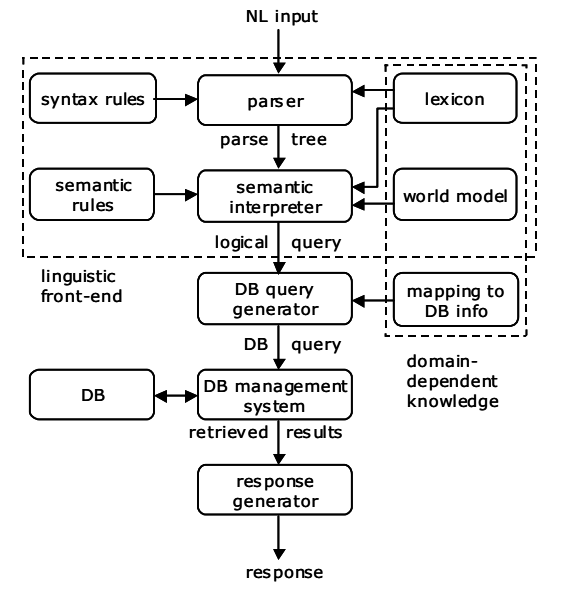
\includegraphics[width=\linewidth]{media/tradi.png}
\caption{Traditional NLP stack (from \cite{andrenucci2005automated})}
\label{fig:tradi}
\end{figure}
\end{center}

\subsection{Problem Formulation}
The focus of this research is question answering in the context of text comprehension. We formulate the definition of the problem as follows: 
\begin{center}
\textit{Given one or more \textbf{natural language documents} containing a number of \textbf{facts} and a natural language \textbf{question}, find relevant facts in the input documents, perform necessary reasoning over the facts, and present the \textbf{answer} in either structured or natural language format.}
\end{center}

The above definition requires a QA system to be able to take natural language information sources and queries as input and perform at least simple logical inferences to extract the answer desired. Unlike information retrieval tasks, in text comprehension tasks, we usually restrict the allowed information sources to the input documents only.

In the context of cross-lingual transfer learning, we wish to solve this problem in one language, and use the knowledge learned in the source language to assist the training of a model on a target language, using documents and Q\&A pairs from both the source and target language.

We may simplify the transfer learning procedure as follows:

Let $L_1$, $L_2$ be two languages, $C_1$, $C_2$ be documents from the two languages respectively, $Q_1$, $Q_2$ be the questions and $A_1$, $A_2$ be the answers.

We learn a model on $L_1$:
\[  M_1(C_1, Q_1) \to A_1\]
Then we use $M_1$ and the $L_2$ data to learn a model in $L_2$, taking into account the shared knowledge with the same task in $L_1$:
\[  M_2(C_2, Q_2 \vline M_1) \to A_2\]

In later chapters we will also consider the cases where $M_1$ and $M_2$ are combined in the same model.


\section{Current Research in Neural QA}

While the traditional NLP systems often employ a rule-based system for parsing inputs and generating outputs, recent neural network-based NLP systems usually attempt to build a distributional model of the language and use that as a basis for solving various problems. The rise of deep neural networks sparked a whole new round of research into natural language processing. Specifically, the effectiveness of recurrent neural networks at sequence processing and the surprising usefulness of embedded word vectors enabled the direct (sometimes even end-to-end) application of neural network-based models in relatively complex NLP tasks such as sentence parsing, transcription, translating as well as question answering. In this section, we discuss the key concepts and techniques used in neural network NLP relevant to text comprehension and multilingual transfer learning.

\subsection{Datasets and Benchmarks}

To compare different question answering techniques as well as to validate the effectiveness of new models, many benchmarking datasets and tools have been developed and adopted by researchers over the years. For instance, the TREC (Text Retrieval Conference) datasets are widely used for information retrieval benchmarking. For text comprehension and reasoning over text data, traditionally there was a lack of large, high quality datasets suitable for the task. In recent years, several new datasets have been proposed to meet these demands. The three sample datasets mentioned below represent three main types of question answering tasks: text-based reading comprehension (the focus of this research), logical reasoning / inference, and open questions.

\paragraph{CNN / Daily Mail }

The CNN / Daily Mail QA dataset was collected by Hermann, et al. \cite{hermann2015teaching} for developing their deep neural network-based question answerers. The  dataset consists of more than 300k articles taken from CNN and Daily Mail websites. Questions on each article are built from the bullet points for these articles. In order to truly test an algorithm for its ability to extract information from the text itself rather than relying on “common sense knowledge” (such as those deduced from word co-occurrence), Hermann et al. also anonymised the named entities in the corpora. 

In Chen, et al. \cite{chen2016thorough}, this dataset is studied for its effectiveness in evaluating text comprehension models. The authors conclude that this dataset is valuable for training QA models, however it has several limitations, such as noisy data, relatively simple reasoning tasks and limited room of improvement for future models. However, since it is relatively easy to construct similar datasets in a different language using the same data collection and preprocessing techniques (no human annotation needed), whereas many more recent, higher quality models are much more difficult to replicate in different languages, we believe this dataset is still valuable for developing cross-lingual transfer learning models.

\paragraph{bAbI} 

The bAbI dataset was constructed by Weston, et al. \cite{weston2015towards} specifically for evaluating a model’s ability to reason over natural language evidences. The dataset generally consists of “stories” in which a set of simple statements are followed by a question based on previous statements. There are a total of 20 different categories of tasks, varying in the number of evidences needed for each question and the type of reasoning required. A sample of the bAbI data is given in figure \ref{fig:babi}.

\paragraph{TriviaQA}

TriviaQA \cite{joshi2017triviaqa} is a new dataset for question answering designed to overcome many of the shortcomings of older datasets, such as dataset scale, evidence type (i.e. type of reasoning required), syntactical variation, vocabulary size, etc. It is constructed by combining trivia questions with supplementary evidence documents collected from web searches and wiki pages. The quality and benchmarking effectiveness of this dataset are yet to be further tested. 

\begin{center}
\begin{figure}
\fbox{\begin{minipage}{30em}
\begin{itemize}
\item[1] Bill went back to the cinema yesterday.
\item[2] Julie went to the school this morning.
\item[3] Fred went to the park yesterday.
\item[4] Yesterday Julie went to the office.
\item[5] Where was Julie before the school? office
\end{itemize}
\end{minipage}}
\caption{bAbI example (from \cite{hermann2015teaching})}
\label{fig:babi}
\end{figure}
\end{center}

\subsection{Neural Networks and Deep Learning in NLP}

\paragraph{Recurrent Network Architectures}
Recurrent neural networks are neural networks with cycles in its connections. Conceptually, the circular connections are usually unrolled and represented as a connection from the network in time step t-1 to t. This allows the network to pass state representations between time steps and therefore capture long-distance relationships within the input sequence. This is essential for NLP, as medium to long-distance dependencies frequently exist in phrases, sentences, and documents. A few modifications to the basic architecture have been designed to decrease the training difficulty and increase the representation power of RNN, such as LSTM \cite{hochreiter1997long} and GRU \cite{cho2014learning}. Frequently, a bidirectional RNN is used to allow information to flow from the end of the sequence back to the beginning. In QA tasks, these designs are commonly used to encode sentences and questions, perform reasoning over facts and generate answer sequences. 

\paragraph{Word Embeddings}
The development of techniques to embed words in a dense lower-dimensional vector space is crucial to almost all types of NLP tasks. Prior to the adoption of these techniques, most NLP processes use one-hot word vectors to represent individual words in a document. This approach has the obvious drawback of being extremely sparse and unable to capture relationships between words. Word embedding generation algorithms such as word2vec \cite{mikolov2013efficient} and GloVe \cite{pennington2014glove} provide us with generic means to create semantically meaningful embeddings for various types of NLP tasks. These embedding techniques exploit the context similarities of words and generate embeddings that usually place semantically or functionally related words close together in the embedded space. 
In addition to these general embedding algorithms, it is also possible to train a task-specific embedding by having a neural network find an optimal embedding for the training objective of the network. This is sometimes preferred when the vocabulary size is relatively small and the training examples are abundant. It is also possible to initialise word embeddings in a neural network with a pre-trained generic embedding such as GloVe and fine-tune the embedding with gradients from task objectives. 

In QA tasks, words are normally considered as the most basic unit of the documents (character-level models are rare as far as we know), therefore a word embedding layer is usually the first layer of a neural network model for QA. In tasks where the vocabulary size is relatively small (such as bAbI), the usefulness of pre-trained word embeddings are limited, as it is easy for the network to learn the function and relationship of the vocabulary in its own embedding layer(s). However, for tasks with a larger vocabulary, especially when certain words may not appear or only appear a handful of times in the training data, and when the training data size is limited, an expressive word embedding layer might be crucial for the generalisation power of the network. 

Another more recent word embedding algorithm is FastText \cite{bojanowski2016enriching}, which utilises sub-word structures such as word roots and suffixes to share representation between similar / related words and "interpolate" word vectors for out-of-vocabulary words. This word embedding algorithm has seen increased use recently and is especially convenient for multilingual tasks, as pre-trained word embeddings already exist for 294 languages.

\paragraph{Phrase and Sentence Representations}
It is often not sufficient to obtain vector representations of natural languages at word level. In almost all NL QA task settings, facts are presented in sentences and paragraphs. There are usually two strategies to convert sentences into vector inputs that can be accepted by a neural network: treating the whole document as a word sequence with separators (including both natural punctuations and artificially inserted dividers), or representing each sentence as a single vector. Both strategies have been used in notable works on text comprehension. For the second strategy, there are more options in how to encode a sentence as a single vector. Weston, et al. \cite{weston2014memory} explored two of the most common techniques for combining words into a single sentence, namely weighted average of word vectors and RNN output over a word vector sequence (more details in the next section).  
Another technique of interest is to exploit the recursive structure of a sentence and apply a tree-CNN on a sentence to recursively encode words into phrases then into sentences, such as used in Kalchbrenner, et al. \cite{kalchbrenner2014convolutional}. There lacks a systematic analysis of whether this type of sentence embedding is capable of improving the performance of text comprehension algorithms, but we suspect that the additional incorporated syntactical information could potentially be useful for tasks with long complex sentences where learning about the syntactical structure would have taken up a significant portion of the network’s capacity. 

\subsection{Question Answering with Neural Networks}

\paragraph{Comparison of Traditional Approaches with Neural Network Methods}
Collobert, et al. \cite{collobert2011natural} proposed an multi-purpose neural network model for four different NLP tasks. Although not engineered carefully to utilise elaborate linguistic features, the model compares competitively with the state-of-the-art non-neural network NLP systems at the time, with some networks reaching within 1\% of the best model. Even though not a question answering model, this demonstrates that neural network models have great potential in natural language modelling and understanding.

In Hermann, et al. \cite{hermann2015teaching} a comparison is made between the performance of traditional symbolic matching models and neural network models in CNN / Daily Mail reading comprehension tasks. The benchmarking shows an average 10\%+ improvement in accuracy of the best neural network models over the best symbolic matching models. 

With more sophisticated model design (such as the architectures mentioned below), deep learning models have managed to exceed the performance of traditional NLP approaches in multiple domains. Apart from the improvement in methodology, the availability of large training data and the increase in computation power has contributed greatly to the rise of neual NLP models, as with other sub-fields of deep learning.

\paragraph{Memory Networks}
One of the most notable works in question answering with reasoning and inference is the Memory Network (MemNN) \cite{weston2014memory}. The main contribution of this research over earlier deep models such as deep LSTM is the introduction of an explicit long-term memory module, allowing information in the network to flow not only from the start of one layer to the end (as enabled by RNN layers), but also from one “scan” of the document to the next, allowing previous states (representing the intermediate result of reasoning) to direct and affect the re-interpretation of the facts at the next time step (via an attention mechanism), thus making multi-step reasoning and fact extraction more viable. 

The memory network model is further improved in Sukhbaatar, et al. \cite{sukhbaatar2015end}, allowing it to be trained end-to-end and to be easily appliable to different tasks. In this version of the network, it is able to be trained to map a couple (facts, question) to an answer, which is usually represented as a probability vector over a limited vocabulary. The results on the bAbI dataset from the above two research demonstrate that the Memory Network is capable of performing exceptionally well on multiple types of reasoning tasks, approaching or even reaching zero error rate in some cases, but are still struggling with certain types of tasks such as “positional reasoning” and “path finding” tasks \cite{weston2014memory, sukhbaatar2015end}.

There are still many potential areas of improvement for the Memory Network model, some of which are addressed in later research works (such as the DMN meontioned below). The representation of input sentences and the interaction of questions and facts are achieved with weighed averaging and inner product respectively, which are relatively simple approaches. The memory size of the network determines the maximum number of facts the model is able to process at the same time, which is not efficient when the fact input is long and irrelevant facts have to stay in memory for the entire duration. Despite a lack of further investigation, we suspect that the number of “rescans” (or reasoning layers) in the network is related to the network’s ability to perform multi-step reasoning (it is observed in the results of Sukhbaatar et al. that more “hops” or reasoning layers generally increase the performance on multi-step reasoning tasks). It is difficult to estimate for a given task, how many reasoning layers is optimal, and it is unknown whether the model can trained with variable number of layers.

Other extensions to the memory network include the dynamic memory network (DMN) \cite{kumar2016ask} and key-value memory network \cite{miller2016key}.

\paragraph{Differentiable Neural Computer}
The differentiable neural computer (DNC) \cite{graves2016hybrid} is an external memory-augmented neural network model built to deal with multiple types of tasks in a way more akin to conventional computers. Instead of having the network learn a mapping from inputs to outputs directly, it trains the network to learn a set of operations to manipulate the memory and ultimately to generate the desired output. The network acts as a controller that not only handles input and output, but also issues and receives operations to read and write the memory. The main novelty of this research is the use of differentiable functions in all I/O, operation generation and operation execution steps which enables the training of the network as a whole. 

Graves et al. \cite{graves2016hybrid} have shown in their work that the DNC is capable of learning text comprehension tasks, in this case using the bAbI dataset. The network takes individual word tokens as input (rather than whole sentence representations as in MemNN or DMN) and outputs an answer when a “question end” token is encountered.  An interesting difference between the DNC and previously mentioned models is that there are no explicit reasoning steps or revisiting of facts in the DNC model. The network learns the operations to store memory about the facts in the memory and to construct answers from the memories directly through supervised learning. Intuitively, it works like an active note-taker, who reads the facts, take “notes” about important information in the facts, reads the question, then piece together the answer from previous notes. The DNC is able to achieve lower error rates and task failure rates on bAbI tasks than previous models with only relatively weak performance in two of the tasks.

The DNC is an interesting idea to combine the advantages of conventional and neural computing, and has shown great promise in its ability to solve a diverse set of tasks. It is worth further investigation to explore its application in question answering.

\subsection{Multilingual NLP and Shared Embeddings}

Neural NLP has also been applied to multilingual scenarios. The most obvious application of deep learning in multilingual NLP is machine translation. Most of the current neural machine translation models are based on the sequence-to-sequence encoder-decoder paradigm \cite{kalchbrenner2013recurrent, cho2014properties}, which uses an autoencoder-like architecture to transform input language representations into an intermediate representation ("encoding"), then decode back to natural language representations through a decoder network. Stacked RNNs are typically used for encoding and decoding of word sequences. The common theme of these methods is finding a shared representation of the source and target language as the "interlingua" for the translation task.

Machine translation is regarded as one of the toughest problems in NLP, and thus it is undesirable to rely on machine translation as a preprocessing step for multilingual NLP. There has been several research on enabling multilingual representation sharing and knowledge transfer without the need to perform full machine translation. Since word embedding vectors are typically the entry point of a neural NLP process, finding shared embedded represenations for two or more languages has been an active area of research. Bilingual (or multilingual) word embeddings can be obtained by either aligning the embeddings in the training process, or aligning existing, pre-trained embeddings through projection or fine-tuning. Usually alignment during training are able to produce higher quality embeddings, but such embeddings might be prone to monolingual performance degradation and are more time- and resource-consuming to train. On the other hand, alignment after training might not produce as high performing results in cross-lingual tasks, but it is possible to avoid monolingual performance degradation and they are relatively cheap to compute.

In Gouws and S{\o}gaard, an algorithm to train a bilingual word embedding using an arbitrary base embedding algorithm and a set of equivalence relationships is proposed \cite{gouws2015simple}. During the training of word embeddings, words are randomly replaced with their equivalences with a set probability so that in a sense, equivalences share their contexts. One major benefit of this approach is that it is not dependent on parallel corpora, and the specific equivalence classes used can be chosen to benefit the task (such as using part-of-speech equivalence instead of meaning equivalence to benefit POS tagging)\cite{gouws2015simple}. However, this alignment approach requires that the embeddings be trained for each bilingual pair and each equivalence relation individually.

In Gouws et al. \cite{gouws2015bilbowa}, a different alignment approach is proposed, in which word alignment is not needed. Instead, word embeddings are trained on monolingual data individually and then the dissimilarity data on a smaller, sentence-aligned parallel corpus is minimised. This approach has the benefit of requiring less granularity in its aligned data input as well as providing moderate speedup compared to previous algorithms, however it is still not as fast as fully-offline methods \cite{gouws2015bilbowa}.

A typical offline alignment algorithm ("align after training") is Mikolov et al.'s translation matrix method \cite{mikolov2013exploiting}, in which a transformation matrix is used to project the vector representations of one language so that the distance between the source and target language vectors are minimised on a set of translation pairs. i.e.
\[ \min_W || Wx_i - z_i||^2 \] where $i$ is the index of translation pairs, and $x_i$, $z_i$ are embedding vectors of the i-th word in language 1 and 2 repsectively.

Despite only using a simple linear transformation, this approach is surprisingly effective on top of being cheap to calculate, likely due to the fact that it does not significantly disrupt the linear relationships between monolingual words. A later research by Artetxe et al. found that the distance minimisation objective works best when all word vectors are normalised, and the transformation matrix $W$ is contrained to be orthogonal, as such a treatment perserves the relative distance and position of monolingual word vectors and minimises monolingual performance loss while still achieving good cross-lingual performance boost \cite{artetxe2016learning}. In the latest research on this topic by Artetxe et al., it is found that this offline alignment procedure does not necessarily have to rely on a large set of carefully-selected aligned words, and in the most extreme case, simply aligning the numerals between two languages and gradually expanding the alignment can already achieve reasonable performance \cite{artetxe2017learning}.


\section{Challenges for NLP in Low Resource Languages}

The recent development in neural question answering systems have paved the way to a future of high-performance question answering systems. However, like many other deep learning-based solutions, these systems have one bottleneck in common, namely the availability of high-quality, high-volume training data. Unlike traditional NLP systems whose rules are manually designed by experts, neural NLP systems have to learn its lingustics knowledge and world knowledge from a large amount of input data. It is suggested that in certain NLP tasks, more than a million training examples are needed for the network to reach optimal performance \cite{banko2001mitigating}. 
For question answering tasks, the datasets usually require human annotation, which increases the difficulty of compiling them significantly. Actually one of the first large text comprehension datasets for neural QA benchmarking, the CNN/Daily Mail dataset, circumvents the issue of human annotation by constructing questions from existing news headlines \cite{hermann2015teaching}, which significantly increases the quantity of the data that can be utilised, but also limits the quality of the final dataset. The CNN/Daily Mail dataset contains 380K QA pairs in the CNN section and 879K QA pairs in the Daily Mail section, making it one of the largest public datasets in this catagory.

The Maluuba NewsQA dataset \cite{trischler2016newsqa}, which is derived from the CNN / Daily Mail dataset, improves the question and answer quality of the original dataset by human annotation. It has a total size of 120K QA pairs.

Another frequently used dataset in recent research, the SQUAD dataset \cite{rajpurkar2016squad}, contains over 100K QA pairs.

Almost all of the current QA datasets for machine learning research are in English with a few exceptions, but even these few datasets in other languages are usually
limited by data quantity or quality. The sheer size of the dataset required to train a performant QA system (or NLP systems in general) makes it especially challenging to develop a model for a low-resource language. The lack of high-quantity training dataset is even true for otherwise widely-spoken languages such as Spanish and Chinese. However, as we can imagine, the demand for question answering systems in these languages are not necessarily lower than English. This inevitably puts the onus of collecting a sizeable dataset in the target language on the developer of the system, which may be beyond their capabilities.

Since building large datasets for different languages is difficult, it would be immensely helpful if instead of having to individually collect huge amount of data for each language, we could utilise the relative abundance of training data in resource-rich languages to boost the performance of QA systems trained with limited data in a resource-limited language. Therefore we are motivated to consider the use of transfer learning in QA tasks.


\section{Transfer Learning}

If we consider two text comprehension tasks on two different languages, they are not entirely independent. There exist two main sources of information that can be shared between the tasks:
\begin{itemize}
	\item[1] The languages themselves have some common linguistic features that can be exploited, such as words with equivalent meanings, similar syntactical structures in two languages, etc.
	\item[2] The task itself may require the same logical steps to complete, regardless of the language of its input and output.
\end{itemize}

Therefore, in order to reuse the knowledge learned in a resource-rich language, we consider possible ways to exploit task similarities in these two aspects.

For exploiting similarities between two languages, the most straightforward approach is to increase the similarity of the representations of words from the two languages. We therefore explore the possibility of \textbf{aligning the word embeddings} of the two languages so that similar-meaning words in two languages may have similar vector representations.

For sharing common knowledge for the same task, we consider \textbf{reusing (or sharing) the same network / network layers} between two tasks, so that the network may learn to perform a certain function (such as context matching or reference resolution) on the resource-rich language and generalise it to the resource-limited language. 

Generally, for transfer learning in neural networks, there are two basic approaches, namely fine-tuning (sequential training) and joint training (simultaneous training). The effectiveness of each strategy varies from task to task. In this research we consider both approaches and compare their performance in cross-lingual transfer learning.


\section{Data Collection}

For the purpose of transfer learning and performance comparison, we require two comparable corpora in two different languages with their associated QA pairs. However, as mentioned ealrlier in chapter 4, such datasets are not readily available. Therefore, it is necessary to compile a new bilingual dataset for our experiments. Construction of a human-annotated dataset is outside the scope of this research, but the same methodology used in the compilation of the CNN / Daily Mail dataset \cite{hermann2015teaching} is capable of constructing a reasonably accurate QA dataset from raw news articles without the need of human annotation. For our experiments, we use the CNN section of the CNN / Daily Mail dataset as the English corpus, and compile a new dataset in Spanish following the same methodology.

\subsection{Data Collection Strategy}

In Herrmann et al. \cite{hermann2015teaching}, the QA pairs are generated from news articles with several bullet points. Usually the bullet points on news websites are summary of one of the main topics of the article. By removing one of the key words in a bullet point and requiring the QA system to find best matching word from the article to fill in the blank, we are essentially creating a reading comprehension question for the given article. However, usually only questions generated by replacing unique entities result in meaningful reading comprehension questions, whereas questions generated from replacing common words could often be answered by applying grammatical rules or learning common collocations, therefore the question generation is based on the removal of named entities only. To generate a question from a news article, the bullet points and the news story (content body) is separated and paired up, then one of the named entities in the bullet point is replaced with a \textbf{@placeholder} marker to generate a question about the news story.

To further ensure that the system actually learns to perform reading comprehension rather than simple blank word deduction based on collocation (Such as automatically deduce "Olympics" from having "Rio" as the pervious word), in Hermann et al. \cite{hermann2015teaching}, all named entities are replaced with an entity marker \textbf{@entityX} where X is a random or ordinal integer. This percedure can be performed via named entity recognition.

\subsection{Source Corpus Compilation}

\begin{center}
	\begin{figure}
		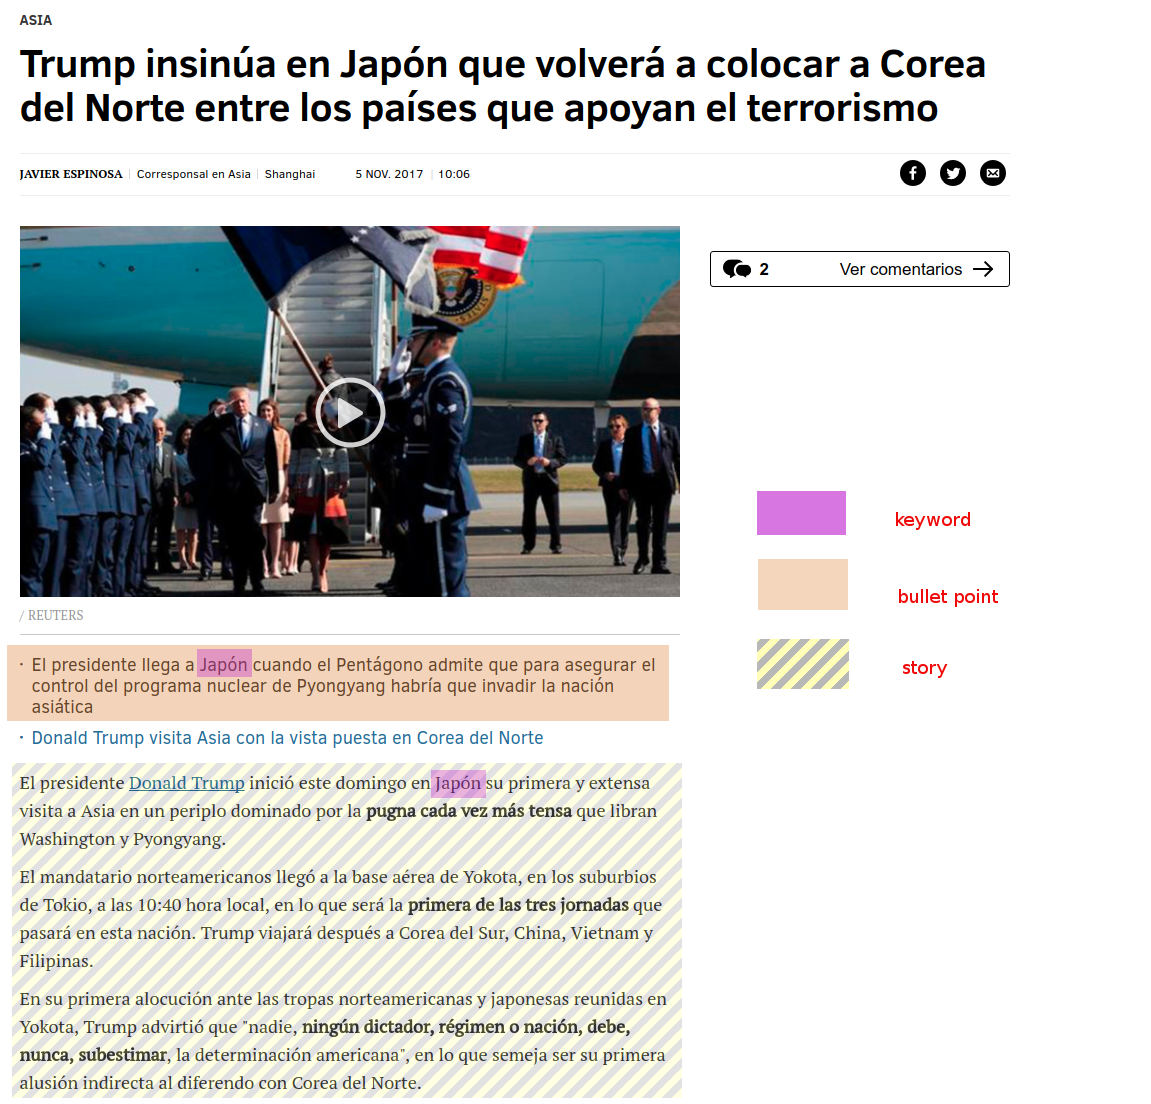
\includegraphics[width=\linewidth]{media/article.png}
		\caption{Example of Scraped Web Page from El Mundo (from \cite{elmundosample})}
		\label{fig:article}
	\end{figure}
\end{center}

\begin{center}
\begin{figure}
\fbox{\begin{minipage}{30em}
\paragraph{bullet points}
\begin{itemize}
\item Mónica Spear y su marido fueron asesinados en presencia de la hija de ambos de 5 años 
\item Han detenido a 7 personas intregrantes de la banda "Los Sanguinarios de El Cambur" 
\item Venezuela tiene una gran tasa de criminalidad: 39 asesinatos por cada 100.000 habitantes 
\end{itemize}
\paragraph{story}
Esta semana Venezuela ha recibido una noticia que ha causado gran consternación en todo el país: el asesinato de la actriz, modelo y ex Miss Venezuela Mónica Spear y de su esposo, el irlandés Thomas Henry Berry . 
El fatídico hecho se produjo en una autopista Venezolana cuando el matrimonio se disponía a regresar a su casa. En el interior del vehículo, se hallaron los cuerpos sin vida de la joven pareja y a la hija de ambos, de 5 años que también resultó herida.
Miles de personas acudieron al velatorio de la pareja. Tanto artistas como familiares y allegados de la actriz y el empresario europeo acudieron desde el mediodía al Cementerio del Este de Caracas para dar el último adiós a la pareja.
...
\end{minipage}}
\caption{Collected Spanish Corpus Sample}
\label{fig:escorp}
\end{figure}
\end{center}

To prepare a dataset in Spanish following the same format, we scrape a total of 37.7K news articles from El Mundo (www.elmundo.es) and CNN Spanish (cnnespanol.cnn.com). The links for news articles from 2014 to 2017 are obtained from historical versions of the front page and categorical portal pages of the websites archived at Wayback Machine (archive.org/web). The articles are filtered to remove video- / picture-only pages and pages only containing extremely brief text (less than 50 words) as well as articles longer than 2000 words for content validity and consistency. The articles are stored as (url, story, bullet point) tuples and duplicated articles are removed. An example of an article before being processed can be seen in figure \ref{fig:article}. Another example from the collected news article corpus can be seen in Figure \ref{fig:escorp}.

\subsection{Data Preprocessing for QA Task}

\begin{center}
	\begin{figure}
	\fbox{\begin{minipage}{30em}
	\paragraph{questions}
		\begin{itemize}
			\item @placeholder y su marido fueron asesinados en presencia de la hija de ambos de 5 años
			\item Han detenido a 7 personas intregrantes de la banda "@placeholder"
			\item @placeholder tiene una gran tasa de criminalidad: 39 asesinatos por cada 100.000 habitantes
		\end{itemize}
	\paragraph{answers}
	@entity10, @entity1, @entity12
	\paragraph{story}
	Esta semana @entity12 ha recibido una noticia que ha causado gran consternación en todo el país: el asesinato de la actriz, modelo y ex @entity8 @entity10 y de su esposo, el @entity13 @entity6 . El fatídico hecho se produjo en una autopista Venezolana cuando el matrimonio se disponía a regresar a su casa. En el interior del vehículo, se hallaron los cuerpos sin vida de la joven pareja y a la hija de ambos, de 5 años que también resultó herida.Miles de personas acudieron al velatorio de la pareja.
	...
	\end{minipage}}
	\caption{Generated Spanish QA pairs example}
	\label{fig:esqa}
	\end{figure}
\end{center}

To match the entity anonymisation used in the CNN / Daily Mail dataset, we also perform entity recognition and replacement in the Spanish corpus. Named entity recognition is performed via the Google Cloud Natural Language API (https://cloud.google.com/natural-language/) and a list of named entities (including unique names, locations and organisations) are generated for each (story, bullet point) pair. For each (story, bullet point) pair, matched entities (such as the full name and abbreivations of the same organisation, or full name and last name of a person) are replaced with the same entity marker. Finally, one of the replaced entities in the bullet point is replaced with the \textbf{@placeholder} marker to generate the question. One bullet point may be used to generate multiple questions if it contains more than one entity from the story. We generate a total of 76K QA pairs via this process. An example of generated QA pairs can be seen in figure \ref{fig:esqa}.

\subsection{Word Embeddings}

In order to compare the transfer learning performance of the networks using unaligned word embeddings and aligned word embeddings, we need individual embedding vectors for both English and Spanish, as well as the aligned versions of these embedding vectors. In our experiments, we use the pre-trained 300-dimensional FastText embeddings \cite{bojanowski2016enriching} due to its large training corpus (Wikipedia) and availability for both languages. For embedding alignment, we use the algorithm outlined in Artexte et al. (2016) \cite{artetxe2016learning} to calculate aligned embeddings via orthogonal transformation (details in the next section). For the aligned vocabulary dictionary needed for embedding mapping, we use the alignement dictionary of OpenSubtitles 2012 parallel text dataset \cite{TIEDEMANN12.463}, available on the Open Parallel Corpus website (http://opus.lingfil.uu.se/index.php). The original FastText embedding vectors for English and Spanish exceed 6.6G and 2.6G respectively, and are thus required to be trimmed to the subset of words that are present in our news article QA datasets. The trimmed version of the embedding vectors are 210MB and 260MB respectively and can be easily handled with our existing experiment setup.



\section{Proposed Solutions and Model Description}

We propose two network architectures for implementation of cross-lingual transfer learning. The first approach relies on sequential transfer learning and use fine-tuning of models trained on a resource-rich language as the main technique of model adaptation. We also apply word embedding alignment as an additional technique of knowledge sharing. The second approach relies on the joint training of models on two languages simultaneously to directly share intermediate representations of the network. In order to encourage the network to learn a truly shared representation for both languages rather than learning two representations in the same network, we also experiment with adding a penalty term optimised via adversarial training.

\subsection{Base QA Model}

\begin{center}
	\begin{figure}
		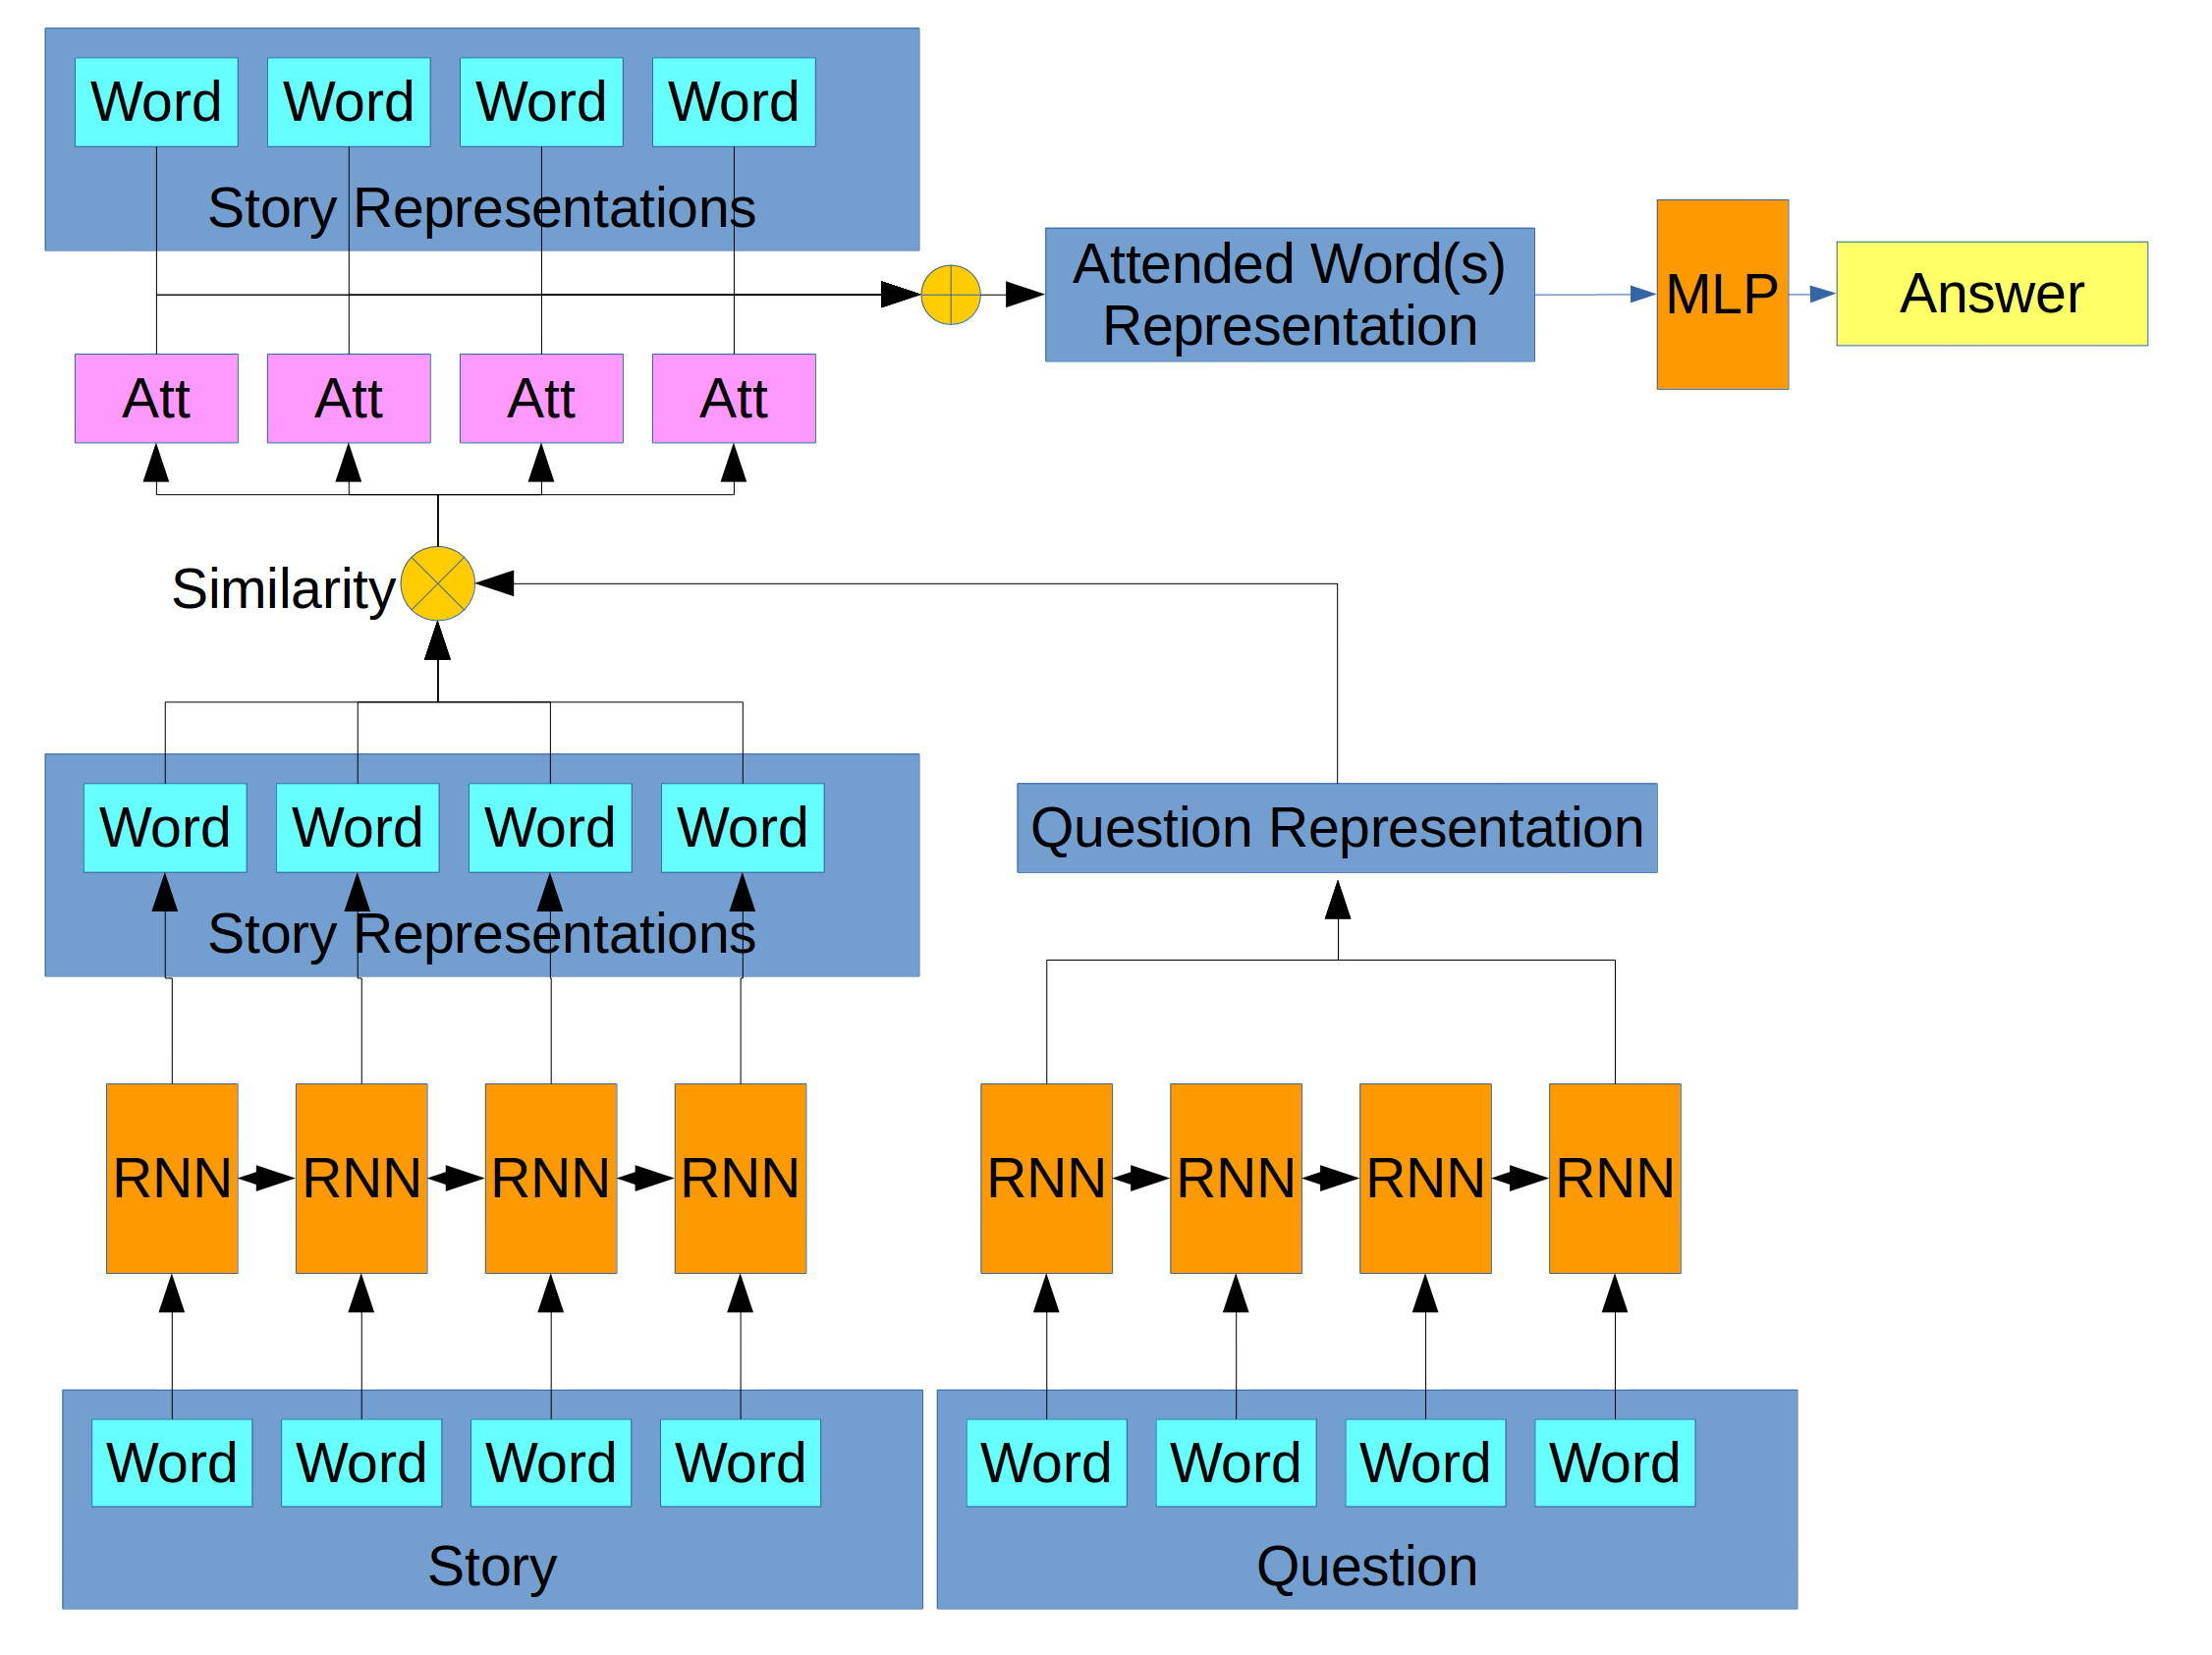
\includegraphics[width=\linewidth]{media/attentive.png}
		\caption{Modified Attentive Reader (based on Hermann et al. \cite{hermann2015teaching} and Chen et al. \cite{chen2016thorough})}
		\label{fig:attentive}
	\end{figure}
\end{center}

For the base monlingual model for question answering, we adopt the improved attentive reader model described in Chen et al. \cite{chen2016thorough}. A basic outline of the network can be seen in figure \ref{fig:attentive}. The network applies two bidirectional RNNs on the embedding vectors of words in the story and question respectively, obtaining individual context-dependent word representations for each word in the story and a summary representation for the question. A similarity score is calculated between the representations of story words and the question to calculate the attention score of each word. A weighed sum of the story word representations (weighed by their attention scores) is then calculated to obtain the representation of the attended word(s). Finally, one or more dense layers act as the classifier to map the attended word(s) representation to the one-hot representation of the answer. The model can be formulated as follows:

\textit{Let $C_i$ be the i-th word in the story, and let Q be the question. Let $R_i$ be the context-dependent representation of $C_i$ and $r$ be the summary representation of the question. We use $a_i$ to denote the attention score, $u$ to denote the attended word representation and $o$ the answer's class. $M$ is a matrix parameter in the bilinear term $R_i^T M r$ to add more expressiveness of the similarity function (as compared to simpler similarity measures like dot product), as suggested by Chen et al. \cite{chen2016thorough}.}

\[ R_i = \phi_{RNN}^C(emb(C_i))[:] \] 
\[ r = \phi_{RNN}^Q(emb(Q))[-1] \]
\[ a_i = Softmax(R^T M r) \]
\[ u = \sum_i a_i R_i \]
\[ o = Softmax(\phi_{Linear}(u)) \]

In practice, this model performs by matching the context in each story position with the question representation, find the positions that best match the \textbf{@placeholder} token's context and focus its attention on these positions. The weighed sum step evaluates the attention received by each position and finds the position with the maximum attention, which is assumed to be the position of the answer token. The final dense layer(s) then map the representation of the answer token (if the attention mechanism finds it correctly) back to its class (i.e. ID of the answer keyword).

\subsection{Sequential Transfer Learning}

In sequential transfer learning, we first learn a model on $L_1$:
\[  M_1(C_1, Q_1) \to A_1\]
Then we fine-tune the trained model $M_1$ on the $L_2$ data to adapt the model to $L_2$:
\[  M_1'(C_2, Q_2) \to A_2\]
where $M_1'$ is initialised with the parameters of $M_1$ and trained with lowered learning rate.

In the most basic form of sequential transfer learning, the model is identical to the base monolingual QA model, except it is trained twice on two different languages. The intuition is that the weights of the network encode information about how to find a proper context-aware representation for word and phrases (mainly via the biRNN layer), as well as how to perform context matching and how to map attend entities back to answer word classes. Only the first step (calculating context-aware representations) is highly language-dependent, whereas the following steps can be though of as language-independent in the abstract sense. Therefore by fine-tuning the network, it should ideally "forget" about the language-dependent functions and retain the ability to perform the language-independent steps.

We may also align the word embeddings so that similar words in the two different languages are represented by word vectors that are close to each other in the shared embedding space. In this way, we may reduce the distance between the representation of similar expressions in $L_1$ and $L_2$, and in turn hopefully reduce the difference between optimal weights of the network for $L_1$ and $L_2$. Perfect word embedding alignment of two languages is not possible, as it is equivalent to solving machine translation, which is an immensely difficult task. By applying the vector alignment technique introduced by Artetxe et al. \cite{artetxe2016learning}, it is possible to minimise the difference between two sets of word embeddings for a selected list of words. It is suggested in \cite{artetxe2016learning} as well as \cite{duong2017multilingual} that such an alignment procedure is also capable of aligning words outside of the alignment dictionary via the preservation of relative position of an arbitrary word relative to these "anchor" words, as discussed in chapter 3. Therefore, we may use the following objective to find the best projection for aligning two word embedding matrices:
\[ arg\min_P ||PX_1 - X_2|| \]
where P is an orthogonal matrix.

We may then formulate the shared embedding model as follows:

Define:
\[ \phi(\cdot)=\phi^{RNN}((\phi^{word\_emb_{L_1, L_2}}(\cdot) + \phi^{entity\_emb}(\cdot)) \]
\[ \sigma(R, r)=softmax(R^T M r) \]

Then:
\[ R_i^{(j)}[:]=\phi^{(C)}(C_i^{(j)})[:] \]
\[ r_i^{(j)}=\phi^{(Q)}(Q_i^{(j)})[-1] \]
\[ \gamma(R, r) = Softmax[Linear(\sigma(R, r)^T R)] \]

And the training objective can be defined as:
\[ argmin_{\Theta_\phi, \Theta_\gamma, \Theta_\sigma} -logP(A|Q, C, \Theta_\phi, \Theta_\gamma, \Theta_\sigma) \]
We use $\Theta$ to denote the parameters for a certain network.

\subsection{Joint Learning with Adversarial Training}

In the joint learning approach, we train the same model to perform the same QA task in both languages. We have only one model:
\[ M(C_i, Q_i) \to A_i \]
where $i$ can either be 1 or 2. 

In its most basic form, the network architecture is also identical to that of the base monolingual model, and the only difference is in the composition of the training examples. The network now takes a random mixture of training examples from two languages and has to predict the answer regardless of input language. For the simple joint training case, we use aligned word vectors as in the last section to increase task similarity between two languages.

Two of the main challenges of joint training a network on two tasks are:
\begin{itemize}
	\item[1] If the network is too expressive (having more parameters than optimal), the network might overfit and learn two separate modes for two different tasks, undermining the whole point of joint training.
	\item[2] If the network is not expressive enough, the network might fail to learn a useful shared intermediate representation for the two tasks, learning a set of "average weights" that perform well on neither tasks.
\end{itemize}

To avoid these issues, we have to find a way to encourage the network to share intermediate representations between tasks, or equivalently, penalise the network for using significantly different representations for separate tasks. Suppose $R^*$ is an ideal shared representation between tasks in $L_1$ and $L_2$, we wish to find a penalty term similar to the following form:
\[ -\alpha (||R^* - R_1|| \cdot I_{L_1} + ||R^* - R_2|| \cdot I_{L_2}) \]
(Here the $R$'s do not strictly correspond to the $R_i$'s in the base model. They may correspond to intermediate representations from $R_i$ and $r$ to $u$ in the orignal model, depending on implementation details, but the idea is the same: share representation between two tasks at some level of the network.)

In other words, a penalty term that penalises the network for adopting an intermediate representation that is too different from the ideal, shared representation. However, such a penalty function does not readily exist because we cannot know the ideal shared representation $R^*$ beforehand. However, we do know that if $R_1$ and $R_2$ deviates from $R^*$ too much, they will be different from each other, and if the average of $||R_1 - R_2||$ is significant, a discriminator network can be trained to distinguish them from each other and determine their source language just by looking at these intermediate representations. Therefore it is possible to train a discriminator network whose performance score can serve as the penalty term for not sharing representations.

We may formulate the network with the discriminator included as follows (choosing the attended word representation layer $u$ for applying the discriminator):

(Same definition for $\phi(\cdot)$ and $\sigma(\cdot, \cdot)$ as above)
\[ R_i^{(j)}[:]=\phi_i^{(C)}(C_i^{(j)})[:] \] 
\[ r_i^{(j)}=\phi_i^{(Q)}(Q_i^{(j)})[-1] \]
\[ u = \sigma(R, r)^T R \]
\[ \gamma(u) = Softmax[Linear(u)] \]
\[ \delta(u) = \delta^{MLP}(u) \]

One challenge of training this network is that it has multiple objectives. The primary objective is to minimise the loss of the answerer network $\gamma$, but the answerer network also has to take into account the penalty term and lower the accuracy (i.e increase the loss) of the discriminator network. However, in the mean time, the discriminator network also has to be trained, and its weights should be optimised to lower the discriminator loss. These objectives are at odds with each other. Fortunately, it is possible to combine the training objectives of the answerer network and discriminator network together and simultaneously update their weights following opposite gradient directions, using an adversarial training technique introduced by Ganin et al. \cite{ganin2016domain}.

\begin{center}
	\begin{figure}
		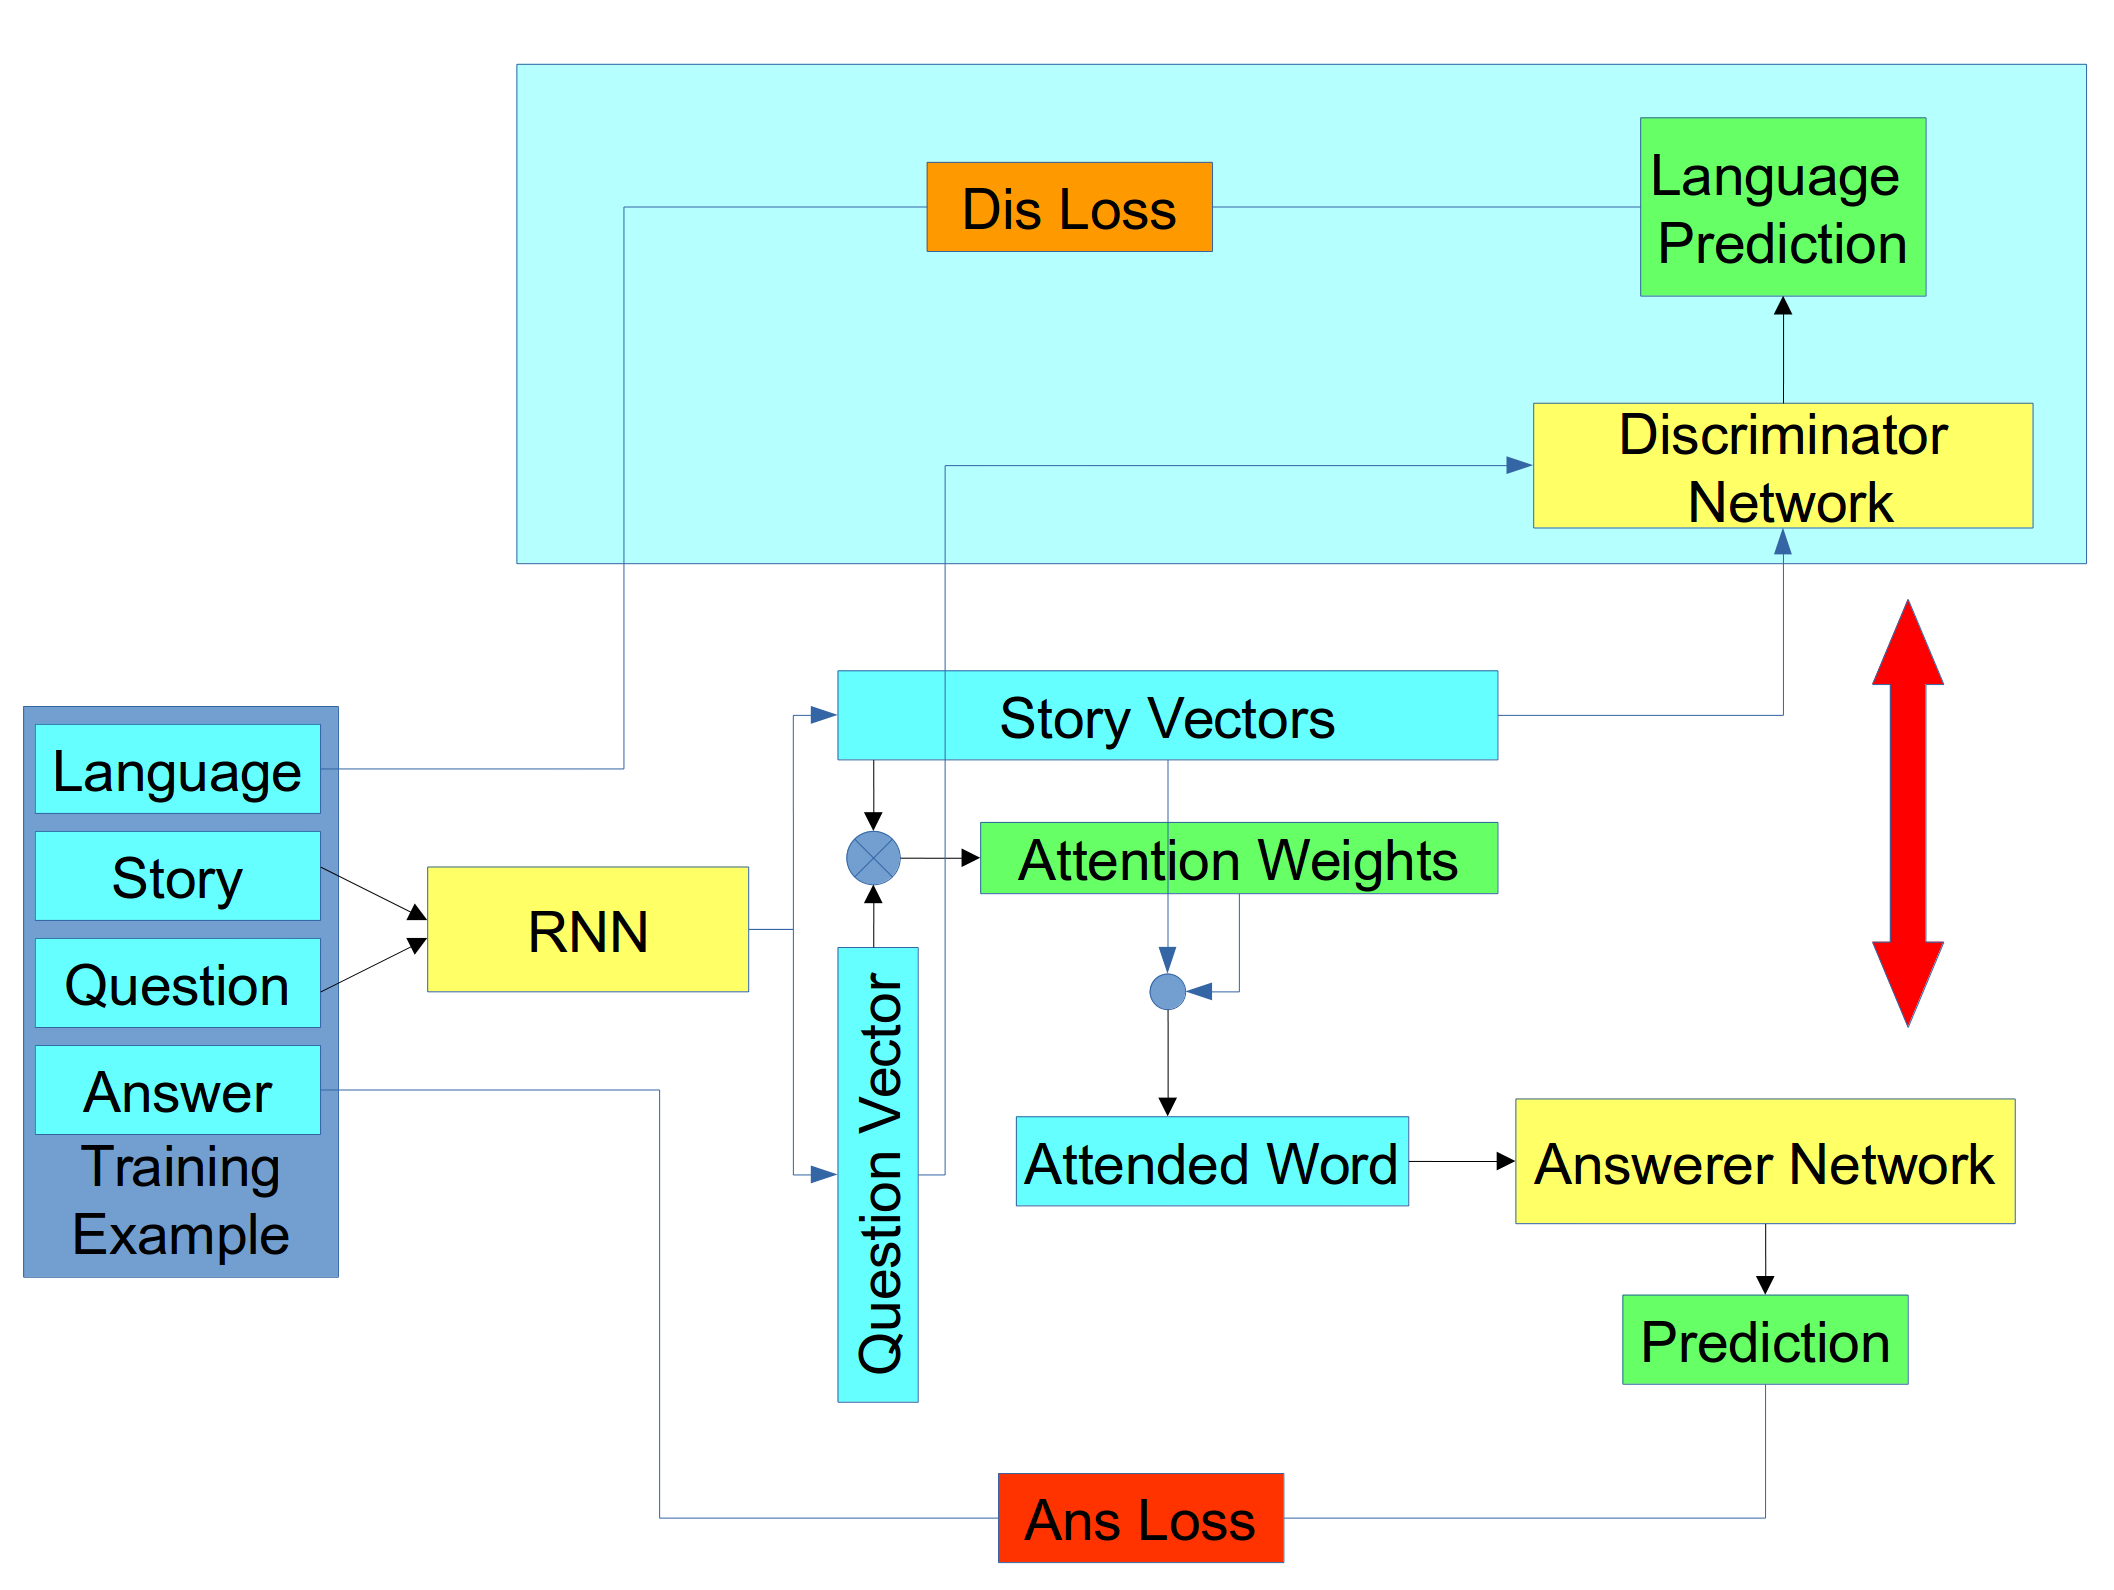
\includegraphics[width=\linewidth]{media/adversa.png}
		\caption{Modified Attentive Reader with Adversarial Training}
		\label{fig:adversa}
	\end{figure}
\end{center}


We may write the joint training objective as follows:
\[ argmin_{\Theta_\phi, \Theta_\gamma, -\Theta_\delta} [-logP(A|Q, C, \Theta_\phi, \Theta_\gamma) + \alpha \cdot log P(\lnot L|Q, C,\Theta_\phi, \Theta_\delta)] \]
(we include $\Theta_\sigma$ in $\Theta_\phi$ for clarity)

Notice that $\Theta_\phi$ and $\Theta_\gamma$ are parameters of the answerer network (part of the network in the base model), whereas $\Theta_\delta$ is the parameters of the discriminator network. This training objective follows the gradient of the answerer network weights to minimise answerer loss and maximise discriminator loss, and also simultaneously follows the negative gradient of the discriminator network weights to minimise the discriminator network loss. Intuitively there exists a competition between the answerer network and the discriminator network, where the discriminator network strives to best classify intermediate representations by their language, and the answerer network tries to confuse the discriminator network by outputing similar-looking intermediate representations. In this way, we are able to encourage the answerer network to produce an intermediate representation that shares as much information as possible between tasks from the two languages. The combined architecture of the answerer and discriminator network is shown in figure \ref{fig:adversa}.

\section{Experiments}

\subsection{Experiment Setup}

The network architectures from the previous chapter are implemented in PyTorch 0.2. For word embeddings, we use the trimmed version of the pre-trained 300-dimensional FastText vectors provided in \cite{bojanowski2016enriching} and their aligned versions, as described in the "Data collection" section. For words in the news articles that do not have an existing embedding vector, we map them to one of the 100 randomly generated embedding vectors (all instances of the same word are mapped to the same vector). For entity tokens and placeholder tokens, we also map them to random embedding vectors sampled from a normal distribution. All embedding vectors in our experiments are normalised to length 1. Throughout our experiments, we do not perform fine-tuning on embedding vectors and use them as is. (Main reason for this is that fine-tuning on the embedding vectors would expose the answerer network to the language label of the input indirectly in the joint + adversarial training case, which is not desirable.)

For our model parameters, we mostly use the same values recommended by Chen et al. \cite{chen2016thorough}. We use a batch size of 32. For the biRNNs, we use a hidden layer size of 128. We apply a dropout rate of 0.2 on the embedding layer output. For the initial training of models as well as joint training, we use the Adam optimiser \cite{kingma2014adam} with a learning rate of 0.001. For fine-tuning, we use Adam with learning rate 0.0001. 

Similar to \cite{chen2016thorough}, we adopt a few additional techniques to improve the model performance: 
\begin{itemize}
	\item Using entity relabeling to label the entities based on their order of appearance. This we believe is potentially implicitly assigning different prior probabilities to entities appearing in different positions in an article. For instance, over time, the network may learn to assign higher answer probability to entities from the beginning of the story, as it is common for news articles to contain main points in opening paragraphs. This entity labeling strategy allows the network to exploit such patterns.
	\item Predicting an answer only in the subset of entities that actually appear in a document.
	\item Using a bilinear term instead of a dot product for similarity measure between the question and contextualised story word representations.
\end{itemize}

The experiments are run on a cluster with nVidia P100 GPUs. The average training time for single language model training takes approximately 2-3 hours before hitting early stopping criteria. Fine-tuning takes 1-2 hours on average. Joint models takes approximately 4-5 hours to converge.

\subsection{Results}



\section{Discussions}



\section{Conclusion}



\section{Future Work}


\newpage
\bibliographystyle{acm}
\bibliography{thesis}


\newpage
\appendix
\section{Appendix}

\end{document}
